\documentclass[12pt]{article}
        \usepackage{graphicx,type1cm,eso-pic,color}
        \usepackage{hyperref}
        \usepackage[left=3.0cm,right=3.0cm,top=2cm,bottom=2cm,headheight=13.6pt]{geometry}
        \usepackage{subfigure}
        \usepackage[mmddyyyy]{datetime} 

\makeatother


\title{Manual for HPS ECal}

\author{Main contact: xxx-xxx-xxxx (ECal cell phone) \\ 
For questions about the manual: \\
General: Rapha\"el \textsc{Dupr\'e} (dupre@ipno.in2p3.fr)\\ 
LED system: Andrea \textsc{Celentano} (andrea.celentano@ge.infn.it)
}

\date{v-21-10-2014}

\begin{document}
\maketitle{}

   \section{General description of the ECal}

\begin{figure}
\center
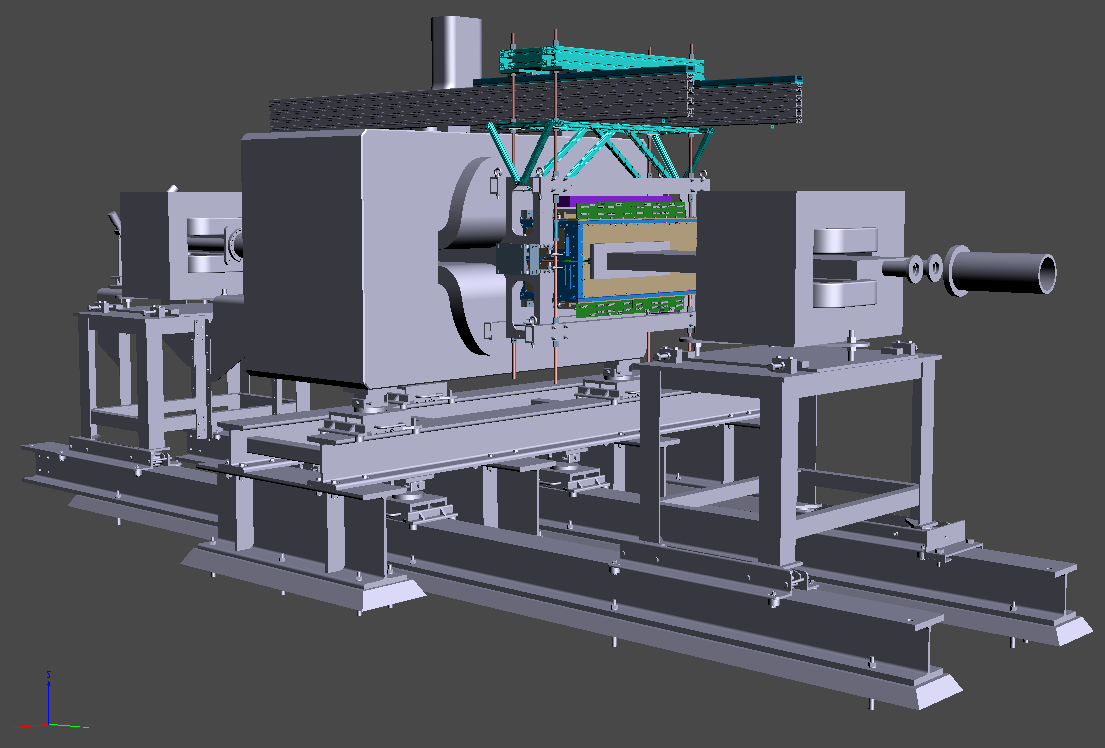
\includegraphics[width=0.75\textwidth]{GView.png}
\caption{\small \label{GView} General view of the ECal (in color) suspended at the downstream end of the HPS analyzing magnet.}
\end{figure}

\begin{figure}
\center
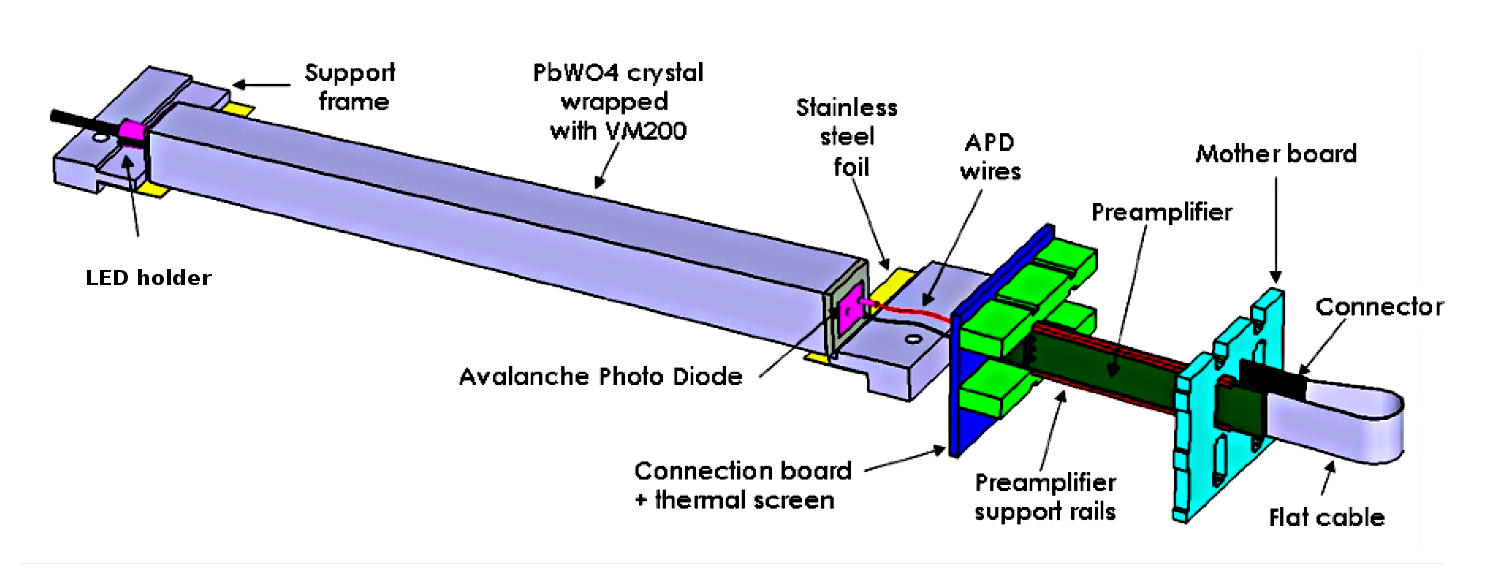
\includegraphics[width=0.75\textwidth]{CrystalAssembly.png}
\caption{\small \label{AmplChain} View of an ECal crystal and the amplification chain.}
\end{figure}
      

The electromagnetic calorimeter (ECal), installed downstream of the pair spectrometer dipole magnet (figure~\ref{GView}), performs two essential functions for the experiment: it provides the trigger signal and helps identify electrons and positrons. The ECal modules are based on tapered 160 mm long PbWO crystal with a 13.3x13.3 mm$^2$ (16x16 mm$^2$) front (rear) face wrapped in VM2000 multilayer polymer mirror film. The scintillation light, approximately 110 photons / MeV, is read out by a 10x10 mm$^2$ Hamamatsu S8664-1010 Avalanche Photodiode (APD) with 75\% quantum efficiency glued to the rear face surface. The low gain of APDs (150 pC/pC) is compensated with custom-made preamplifier boards, which provide a factor of 225 amplification of the APD signal. In front of the crystals, LEDs are installed to send light into the crystals. These are used in order to check the proper functioning of the ECal and provides complementary information to evaluate gain variations in the various channels of the calorimeter (see figure~\ref{AmplChain}).


\begin{figure}
\center
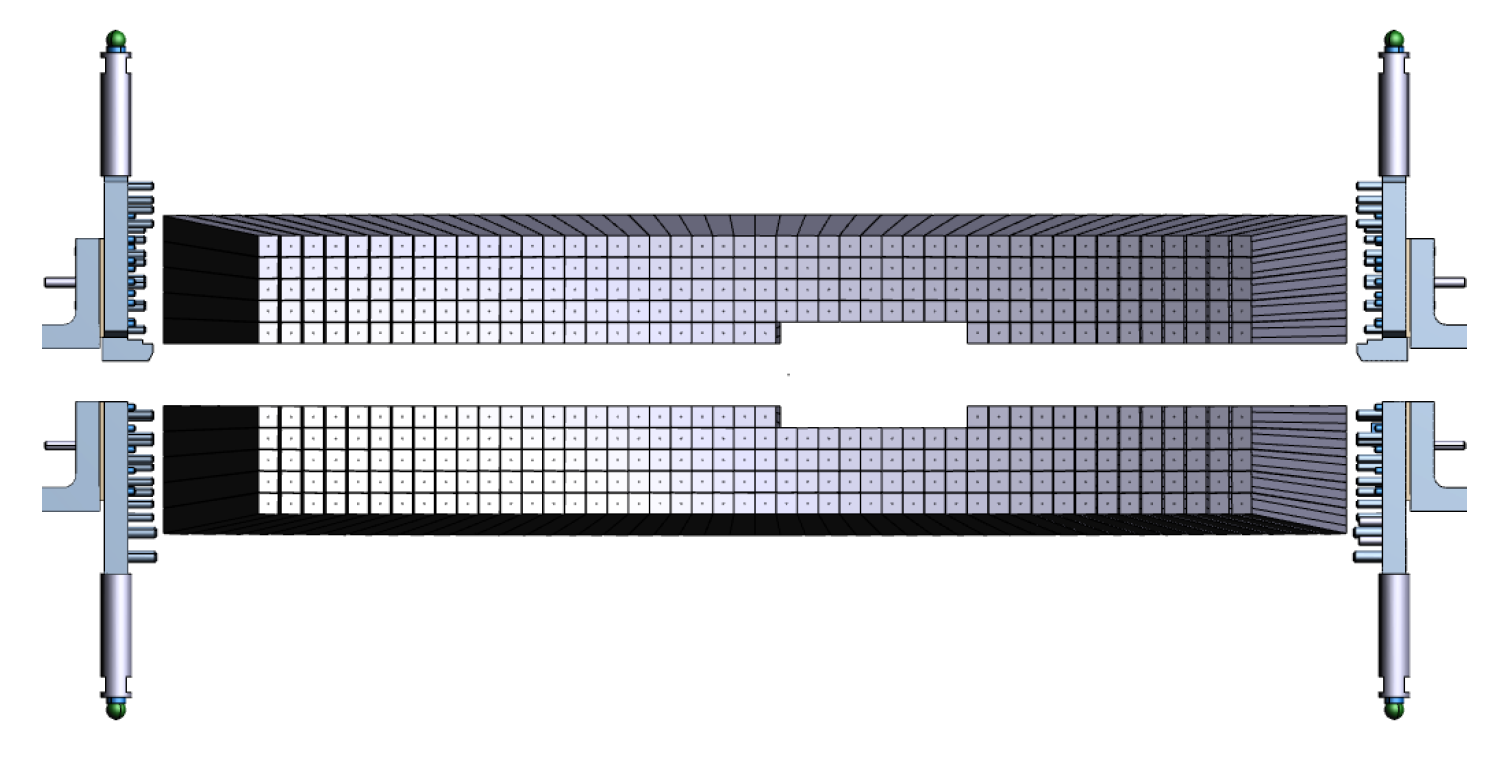
\includegraphics[width=0.75\textwidth]{ECal2.png}
\caption{\small \label{Crystals} Front view of the ECal crystals layout.}
\end{figure}
      
The ECal is built in two separate halves that are mirror reflections of one another relatively to the horizontal plane. The 221 modules in each half are supported by aluminum frames and arranged in rectangular formation with five layers and 46 crystals / layer, except for the layer closest to the beam where nine modules were removed to allow a larger opening for the outgoing electron and photon beams (figure~\ref{Crystals}). Each half is enclosed in a temperature controlled box ( $< 1^\circ$F stability and $< 4^\circ$F uniformity) to stabilize the crystal light yield and the operation of the APDs. Four printed circuit boards (referred as mother boards) mounted on the back plane penetrate the enclosure and are used to supply the $\pm5$ V operating voltage for the preamplifiers, the 400 V bias voltage to the APDs, and to read out signals from the APDs. Each half of the ECal is divided into 26 bias voltage groups formed in order to minimize the gain spread of the APD-preamplifier couples.


After a 2:1 signal splitter, 1/3 of an amplified APD signal is fed to a single channel of a JLab flash ADC (FADC) board. 2/3 of the signal is sent to a discriminator module before a TDC for a time measurement. The FADC boards are high speed VXS modules digitizing up to 16 crystal signals at 250 MHz and storing 4 ns samples with 12-bit resolution. When a trigger is received, the pipeline is read on these boards from 5 samples before and 30 after the trigger time (those values will be adapted during commissioning).



\part{For Shift Takers}

   \section{Slow Controls}

      \subsection{Temperature}

\begin{figure}
\center
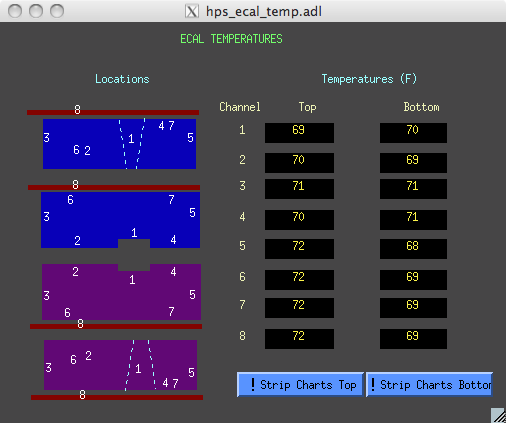
\includegraphics[width=0.75\textwidth]{ECal_temp_monitor.png}
\caption{\small \label{temp} View of the EPICS temperature monitoring window.}
\end{figure}
      
         The ECal temperature should remain as stable as possible in order to avoid gain variation in the system. Eighteen temperature sensors are placed in the ECal enclosure and should be monitored through EPICS (see figure~\ref{temp}). Variations of two degrees F or more during a shift should be reported to ECal expert on call.

      \subsection{Scalers}

         Rates are indicated in the EPICS (Fig \ref{Scalers}) and should remain constant within ~10\% during stable beam operation.

\begin{figure}
\center
%\includegraphics[width=0.75\textwidth]{.png}
\caption{\small \label{Scalers} View of the EPICS HV scalers window.}
\end{figure}

   \section{Turning on/off the ECal}

      \subsection{Turning on}

      Check first that the chiller and the low voltage power supply are on ({\bf The low voltage should always be on before HV.}). These are controlled manually in the hall. Ramp up the HV using the EPICS application (see figure~\ref{HV}).

      \subsection{Turning off}

      Turn off high voltage supply using the EPICS application (see figure~\ref{HV}) then turn off low voltage. The chiller should stay on except for long shutdown, since cooling the ECal takes several hours.

\begin{figure}
\center
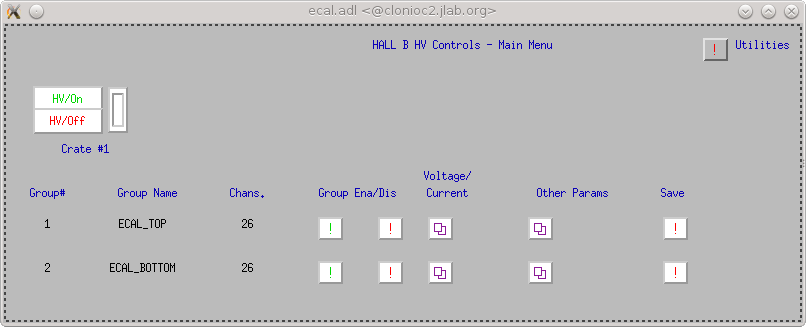
\includegraphics[width=0.75\textwidth]{ecaladl.png}
\caption{\small \label{HV} View of the EPICS HV monitoring and control window.}
\end{figure}


   \section{Responding to HV trips}

      HV trips are indicated by an alarm in the EPICS 
      Record all HV trips in the log book with indication of the group and run number concerned. HV can be turned 
      back on in the same EPICS window. The HV takes around xx (to be updated) to turn back on. If 
      that does not work try again, if still not working ask MCC to turn off the beam and retry. If that is 
      still not working contact the ECal expert on call.

      {\bf If you encounter more than two HV trips during your shift, 
      you should notify the ECal Expert.}

   \section{LED Monitoring}

      \subsection{System setup}

      \textbf{NOTE 1:} At the time of writing of this manual, the EPICS interface is currently under development. Therefore, the instructions reported refer to the operation mode with a direct connection to the controller, using a program such as \texttt{nc} to connect with it and send commands. When the EPICS interface will be available, these operations will be performed directly through it.\\
      \textbf{NOTE 2:} The full list of available commands is reported at the following address: 
      \url{http://wiki.ge.infn.it/g3wiki/index.php/Monitoring_system} 
      (username: clas, password: e1tocome) Only commands to perform ``basic'' operations are reported here. 

      \begin{enumerate}
      \item{Connect to the TOP controller using the \texttt{nc} command. For example, if the IP address of the TOP controller is 192.168.0.2, use:\\
      \texttt{nc 192.168.0.2 9764}}
      \item{Turn it ON, using the \texttt{TURN ON} command.}
      \item{Set the clock to internal, using 1 kHz frequency:\\
      \texttt{SET CLOCK INT}\\
      \texttt{SET FREQ 3}
      }
      \item{On a different shell, connect to the BOTTOM controller using the \texttt{nc} command.}
      \item{Turn it ON, using the \texttt{TURN ON} command.}
      \item{Set the clock to external:\\
      \texttt{SET CLOCK EXT}
      }
      \end{enumerate}

      \subsection{System usage}

      \subsubsection{Get system info}
Here we assume that the system setup is already performed, and that the user is connected via \texttt{nc} to the proper controller (TOP controller if the LED is connected to ECal TOP, BOTTOM controller if the LED is connected to ECal BOTTOM).

      \paragraph{Get system status}

      \texttt{GET STATUS}: returns ON/OFF

      \paragraph{Get clock source}

      \texttt{GET CLOCK}: returns INTERNAL / EXTERNAL

      \paragraph{Get clock frequency}

      \texttt{GET FREQ}: returns the internal clock frequency, in Hz. If the clock source is External, the reported value is meaningless.

      \paragraph{Get LED status}

      \texttt{GET LED\_STATUS n}: returns the status of LED n ($0\leq n<224$). ``1'' if the LED is ON, ``0'' if the LED is OFF.

      \paragraph{Get LED amplitude}

      \texttt{GET AMPLITUDE n}: returns the amplitude setting for LED n.

      \paragraph{Get LED width}

      \texttt{GET WIDTH n}: returns the width setting for LED n.

      \subsubsection{Switch ON/OFF a LED}

      These are the instructions to switch ON/OFF a single LED. Remember that, for each driver board (see map in annex), only one LED at time can be switched ON.
      Here we assume that the system setup is already performed, and that the user is connected via \texttt{nc} to the proper controller (TOP controller if the LED is connected to ECal TOP, BOTTOM controller if the LED is connected to ECal BOTTOM).

      We refer to the LED to turn on as \texttt{n}, with $0\leq n < 224$.

      To switch ON:
      \begin{enumerate}
      \item{Optional: set the LED amplitude, using:\\
      \texttt{SET AMPL n x}\\
      with $0\leq x < 4096$. If this step is skipped, the LED will be turned ON with the amplitude that was last set with this command. If the command was never issued, the default value (1000) will be used.}
      \item{Optional: set the LED color, using:\\
      \texttt{SET COL R}/\texttt{SET COL B}\\
      If this step is skipped, the last color selected for \textbf{any LED on the same driver} will be used. If the command was never issued before, the default color is Blue.}
      \item{Switch ON the LED:\\
      \texttt{SWITCH ON n}
      }.\\
       If there is already a  LED ON on the same driver, the command has no effect.
      \end{enumerate}

      To switch OFF: \texttt{SWITCH OFF n}. If the LED was already OFF, this command has no effect.

      \subsubsection{Set the amplitude setting of ALL LEDs}

      To set the amplitude setting of ALL LEDs connected to a controller to the same value with one command only, use:\\
      \texttt{SET AMPL\_ALL x}, with $0\leq x < 4095$.

      \subsubsection{Set the width setting of ALL LEDs}

      To set the width setting of ALL LEDs connected to a controller to the same value with one command only, use:\\
      \texttt{SET WIDTH\_ALL x}, with $0\leq x < 4095$.


      \subsubsection{Reboot a controller}

      To reboot a controller, use:\\
      \texttt{REBOOT}\\
      Note that after a reboot, the user has to exit from \texttt{nc} and re-connect again to the controller.


   \section{Making a cosmic calibration run}

   To be added later.


\part{For ECal Experts}

   \section{Localization of ECal elements for experts}

{\bf REMINDER:} Since the ECal is within 3 feet of the beam line it needs to be surveyed by RADCON before any work can be done on it.

{\it Location of other elements (electronics, chiller...) in the Hall to be added when ECal is installed.}

   \section{Cooling system}

     The cooling system is using a xxxx chiller that is controlled through EPICS (Fig to be added). The setting should not be modified, the temperature setting should be fixed at 18 degrees Celsius. In case of problem with the chiller contact ??? (who can take care of these in Hall-B engineer group?).

     Add link to manual for manual settings.

\subsubsection{LED position}
\begin{figure}
\center
\caption{\small \label{Chiller} EPICS Window controlling the ECal Chiller.}
\end{figure}



   \section{Changing LV settings}
      Low voltage power supply should be set at $\pm5$V. The low voltage supply might have difficulties to get at this level because of the high current. If that was the case check, with all power supplies off, that all connection are goods. Then contact run coordinator to see if LV power supply addition is possible. 

   \section{Changing HV settings}
      {\bf NOTE:} Changing HV settings should be taken care of in coordination with the ECal group (contact R. Dupre).

      If for some reason some channels were to drop in gain (or increase), it might be necessary to change the HV settings in the expert ECal EPICS control (Fig.~\ref{EHV}). Such a modification will lead to a modification of the gain used by the trigger system, these values need to be both updated at the same time!

\begin{figure}
\center
%\includegraphics[width=0.75\textwidth]{.png}
\caption{\small \label{EHV} View of the EPICS HV expert control window.}
\end{figure}


%   \section{Moving the ECal}
%      {\bf NOTE:} To be done only by Hall-B technical group!
%
%      Tubes of the cooling system have been extended, this should not be necessary for changing preamplifiers anymore. (To be checked when the ECal is installed).

   \section{Disconnection of a Channel and Preamplifier Replacement}
      {\bf NOTE:} This is a lengthy operation and should only be attempted during run with the authorization of the run coordinator.

      One way to recover a HV group that is tripping is to disconnect the faulty 
      channel causing trouble. To do so, you need to find exactly where the 
      channel is! It might be obvious from data, if the channel was already very noisy, else you will have to test the channels of the group one by one.

      First, turn off the ECal (this might not be necessary anymore: then contact engineer on call to 
      have the Hall-B crew move the ECal out), dismount the back panel and push it out of the way 
      (it cannot be completely removed because of the cooling pipes, these should not be disconnected!). Pulling
      the panel will give sufficient access to replace or unplug the preamplifier 
      on the mother board and proceed to tests (Remember that LV should be on before you apply HV). If the group cannot be recovered by 
      replacing or even removing preamplifiers, it is likely that the motherboard is 
      shorted. In this later case a bypass for the HV is necessary. This can be done 
      by the electronics group of JLab (some of the groups of the top ECal are already 
      bypassing the mother board) and should be scheduled with the run coordinator (it takes about half a day) 

      Then you can close back the ECal, turn it 
      back on (LV first!) and check if all HV channels are functioning. After documenting the logbook, inform R. Dupre of 
      any preamplifier replacement, so that the maps on this manual can be updated. 

   \section{LED system for experts}

\subsection{System description}

The LED Monitoring System is made by 3 sub-components:

\begin{itemize}
\item{The Controllers (2x)}
\item{The LED drivers (8x, 4 per each controller)}
\item{The LED connection boards (4x, 2 per each controller, each board connected to 2 drivers)}
\end{itemize}

\subsubsection{The controller}

The LED controller manages the whole system. It provides the master clock, the LV, and the I2C bus to the drivers connected to it. Up to 6 drivers can be connected to the same controller, using Ethernet-like cables with RJ-45 connectors on both ends. All the 8 wires in the Ethernet cable must be connected. The clock can be from an external source (TTL logic) or internal.

The controller provides the interface to interact with the system. The communication is performed via an Ethernet connection: the controller implements a TCP server, listening for incoming connections on port 9764. Only one client at time can be connected to the system. No user authentication or password mechanism is foreseen to connect. When a client is connected, the TCP server accepts commands, in the form of literal strings (see below). \textbf{Commands are case-sensitive.}

Other than using the EPICS interface, a user can interact with the system using the \texttt{nc} command, available on common Linux systems.

\subsubsection{The driver}

Each driver board hosts the digital and analogue circuits used to pulse the LED connected to it. Each driver manages 56 LEDs, in a independent way. However, due to design constrains, \textbf{only one LED on each driver board can be switched on at time.}

The amplitude and the width of the pulse emitted by the LED can be varied independently for each channel, using the commands reported below.
\begin{itemize}
\item{The amplitude parameter can vary between 0 and 4095. The actual LED pulse amplitude is not linear with respect to this parameter, due to the LED intrinsic characteristics.}
\item{The width parameter is very sensitive and must be handled with care. It can vary between 0 and 4095.
\begin{itemize}
\item{If the width is less than a lower threshold ($\simeq$ 2000), the corresponding LED is switched on continuously. This is referred to as ``DC MODE''.}
\item{If the width is higher than an upper threshold ($\simeq$ 3400) the corresponding LED is switched off.}
\item{If the width is in between the two thresholds, the LED is in pulse mode. Due to design constraints, both the width and the amplitude of the optical pulse are proportional to the width setting.}
\end{itemize}
}
\end{itemize}
It is \textbf{highly} suggested that the width parameter is not used during operations, but rather kept fixed at a proper value, to have the LEDs working in pulse mode. A value of $\simeq$ 3000 is fine. 

The ECal expert does not have to configure any of the trimmers mounted on the driver board. This have been already configured to the appropriate value. In case of problem report to A.~Celentano. 

\subsubsection{The connection board and the LEDs}

Each connection board provides the hardware interface between LEDs, mounted in front of the HPS ECal crystals, and the drivers, mounted outside the calorimeter enclosure. The connection boards are populated only with non-programmable components. 

The employed LEDs are: RAPID 56-0352, with two colors (RED/BLUE). Only one color at time can be selected. The color setting is common for all the LEDs connected to the same driver board.

\begin{figure}
\center
\subfigure{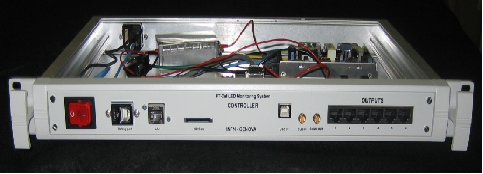
\includegraphics[width=0.45\textwidth]{Controller.png}}\quad
\subfigure{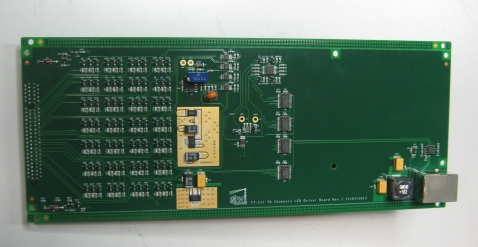
\includegraphics[width=0.45\textwidth]{Driver.png}}
\caption{\small \label{fig1} Left: the main controller. Right: the LED driver.}
\end{figure}


\subsection{Configuration}

In order to have the two controllers synchronized, the following configuration is adopted: the first controller (ECal TOP) generates the master clock from the internal oscillator. This clock is then propagated to the second controller (ECal BOTTOM), that is configured to accept the external clock.

\subsubsection{Default configuration}

When a controller is turned on, these default settings are loaded:

\begin{itemize}
\item{All the LED amplitudes are set to 1000}
\item{All the LED widths are set to 3000}
\item{The LED color is BLUE.}
\item{The clock source is External}
\item{All the LEDs are switched OFF}
\end{itemize}

\subsubsection{LED position}

See figure~\ref{figLED}.

\begin{figure}
\center
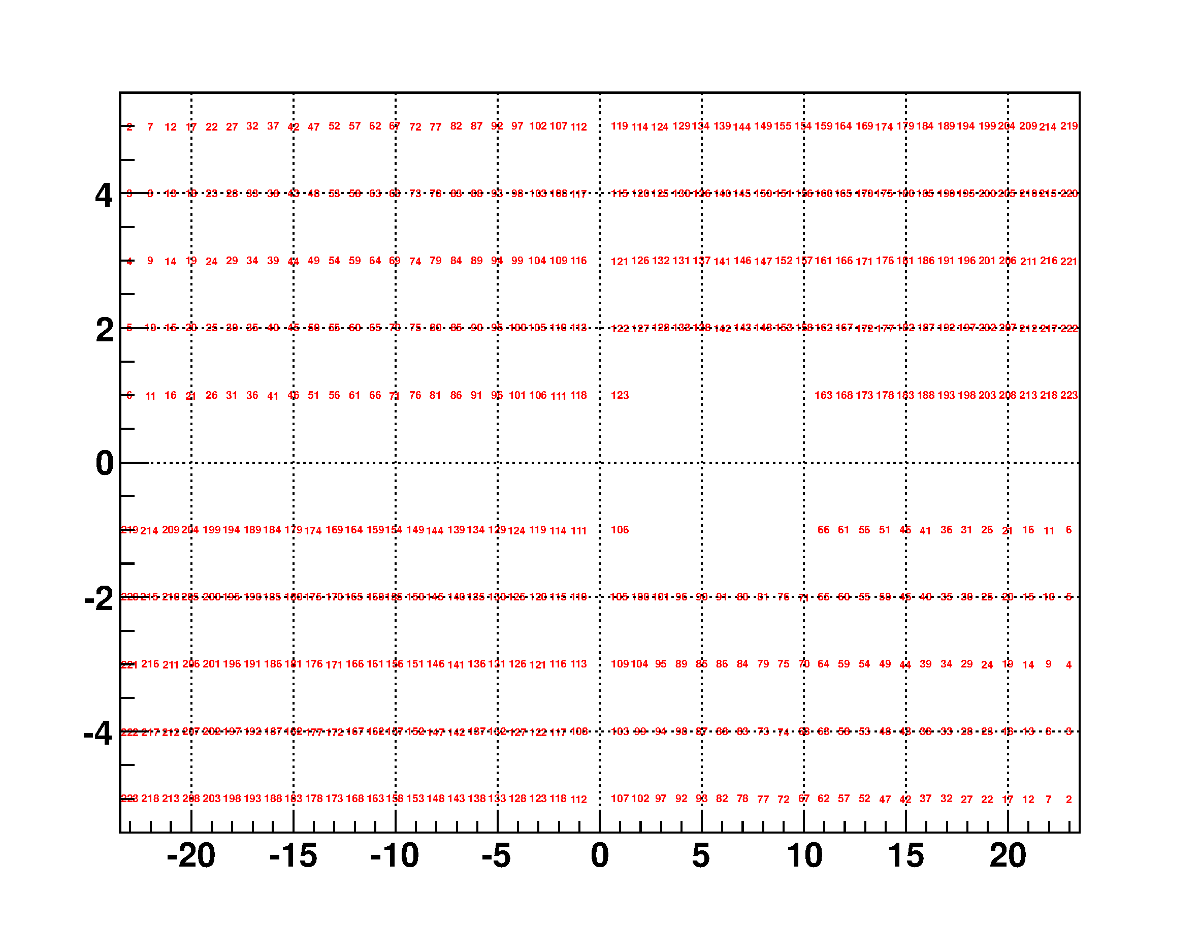
\includegraphics[width=\textwidth]{LedPosition.png}
\caption{\small \label{figLED} Map of the LEDs in the ECal setup (front view). Each number refers to the LED id as in the LED monitoring system.}
\end{figure}

\subsubsection{Operations}

These instructions assume that the LEDs, the connection boards, and the drivers have been already installed by an expert in the ECal setup. They provide a guidance to install the controllers and setup the whole system.

\begin{enumerate}
\item{Optional: install the two controllers in a rack. Each requires 1U space. Install them one on top of the other to minimize the distance.}
\item{Connect the two controllers to the electrical network using the two power cords. The two controllers have been already configured to operate at 110 V, 60 Hz.}
\item{Connect the two controller to the network, using the ``LAN'' connector on the front panel. Each controller requires an IP address provided by a DHCP server. The controller MAC address is written on a label on the front panel.}
\item{Connect each controller to the corresponding 4 drivers using the 4 ``OUTPUT'' connectors on the front panel. Use connectors: 1, 2, 3, 4.}
\item{Use a 2 ns LEMO cable to connect the TOP controller ``SYNC OUT'' to the BOTTOM controller ``Clock IN''.}
\item{Switch on the two controllers using the red switch on the front panel.}
\end{enumerate}


      \subsection{Resolving issues}

      If a faulty channel is found (no signal with the LED system but signal present in data) first try to reboot all the LED system. If that does not fix the problem, some electronics must be changed. The only available option is to replace the driver board with one of the spares, if it fixes the problem contact Andrea Celentano to fix the broken driver board. If this is not the problem, it is probably an issue with the LED or the connection board which cannot be fixed without dismounting partially the ECal, those issues should be documented in the log book and with copy sent to R. Dupre and A. Celentano, these will be taken care of if necessary during long shutdown.

     If larger group of LEDs stop functioning normally, the size of the group should indicate the source of the problem (56 channels correspond to a driver board, half the ECal to the controller board). These should then be replaced with available spares, then contact Andrea Celentano to fix the broken board. In case of unforeseen issues contact R. Dupre and A. Celentano (even if you solved the issue by yourself) so that the problem can be worked out and documented.

      \subsection{Contact person}

      Please report any problem/question regarding the LED system to:\\
\newline
Andrea Celentano\\
andrea.celentano@ge.infn.it\\
+390103536737


\end{document}
